% !TeX spellcheck = cs_CZ
\begin{mdframed}[style=mdexam]
  \begin{example}\label{MAI:exam028}
    Nechť \(\varphi(x) = x^2\), \(a = 1\). Potom \(f(x) = (x^2 - 1 )/(x - 1)\). Pro \(x \neq 1\) je
    hodnota funkce \(f\) rovna \(f(x) = (x + 1) (x - 1 )/(x - 1) = x + 1\). Když \(x \rightarrow 1\)
    (přičemž stále \(x \neq 1\)), pak \(f(x) \rightarrow 2\) (viz obr. 51). Zároveň je také patrný
    charakter tohoto blížení: Hodnoty \(f(x)\) jsou libovolně blízko číslu \(2\), jestliže hodnoty
    proměnné \(x\) jsou dostatečně blízké číslu \(1\). To můžeme říci také takto: 
    
    {\centering
    \captionsetup{type=figure}
  %   % !TeX spellcheck = cs_CZ

\documentclass[11pt]{standalone}
\usepackage{xltxtra}
\usepackage[usenames,x11names]{xcolor}
\usepackage{tikz}
  \usetikzlibrary{intersections}
  \usetikzlibrary{decorations.markings}
\usepackage{pgfplots}
  \pgfplotsset{compat=newest}
\usepackage{amsmath}


\begin{document}
  \begin{tikzpicture}[thick,scale=0.7, 
      every node/.style={transform shape},
      ]
  
  \tikzset{->-/.style={decoration={
    markings,
    mark=at position #1 with {\arrow{stealth}}},postaction={decorate}}}
    
    \begin{axis}[
      xmin = -1.5, xmax = 2.5, ymin = 0, ymax = 3.5,  % osy
      domain = -1:3.5,
      restrict y to domain=0:3,
      axis equal image,
      grid = major,   % both
      grid style={line width=.1pt, draw=gray!20},
      major grid style={dashed, line width=.2pt, draw=gray!40},
      clip = true,
      clip mode=individual,
      xtick={-2,-1,1,2,3,4}, % make steps of length 0.2
      ytick={0,1,2,3,4,5}, 
      axis x line = middle,
      axis y line = middle,
      xlabel={$x$}, ylabel={$y$},
      enlarge y limits={rel=0.07},
      enlarge x limits={rel=0.07}
      ]
      
      \addplot[color=Gold3, samples=10, smooth, ultra thick, unbounded coords=jump, no markers, 
               domain = -1:2.2] 
        gnuplot{x+1}; 
      
      \node [fill=white] at (rel axis cs: 0.9,0.9) {\(y=\dfrac{x^2-1}{x-1}\)};
      
      \draw[line width = 3pt, red, line cap=butt] (0.5,0) -- (1.5,0);
      \draw [thick] (0.5,-.2) node[below] {\(1-\delta\)} -- (0.5,0.1);
      \draw [thick] (1.5,-.2) node[below] {\(1+\delta\)} -- (1.5,0.1);
      
      \draw[line width = 3pt, red, line cap=butt] (0,1.5) -- (0,2.5);
      \draw [thick] (-.2, 1.5) node[left] {\(1-\varepsilon\)} -- (0.1, 1.5);
      \draw [thick] (-.2, 2.5) node[left] {\(1+\varepsilon\)} -- (0.1, 2.5 );
      
      \draw[dashed] (0.5,0) -- (0.5,1.5) -- (0,1.5);
      \draw[dashed] (1.5,0) -- (1.5,2.5) -- (0,2.5);
      \draw[dashed] (1,0) -- (1,2) -- (0,2);
  
      \draw[->-=.5] (1.25,0) node[below] {\(x\)} -- (1.25,2.25);
      \draw[->-=.5] (1.25,2.25) -- (0,2.25) node[left] {\(f(x)\)}; 
       
      \draw[black,fill=white] (1,0) circle (.4ex);
      \draw[black,fill=white] (1,2) circle (.4ex);
      \draw[black,fill=white] (0,2) circle (.4ex);
    \end{axis}
  \end{tikzpicture}
\end{document}
      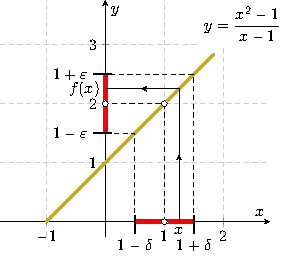
\includegraphics[width=0.45\linewidth]{mai_fig017.pdf}
    \captionof{figure}{K příkladu \ref{MAI:exam028}
    \cite[s.~118]{Brabec1989}
    \label{mai:fig017}}
    \par}
    
    Zvolíme-li libovolně malé okolí bodu \(2\), pak vždy lze najít okolí bodu \(1\) takové, že pro
    každé \(x \neq 1\) z tohoto okolí bude ležet hodnota \(f(x)\) ve zvoleném okolí čísla \(2\).
    Ještě jinak formulováno: K libovolně malému \(\varepsilon > 0\) existuje \(\delta > 0\) tak, že
    pro každé \(x\), pro něž \(0 < \abs{x - 1} \ll \delta\), platí \(\abs{f(x) - 2} < \varepsilon\)
    (viz obr. \ref{mai:fig017}). O funkci \(f\) s touto vlastností říkáme, že má v bodě \(1\) limitu
    \(2\) a píšeme symbolicky \(lim_{x \to 1}f(x) = 2\) nebo \(f(x) \rightarrow 2\) pro \(x
    \rightarrow 1\).
  \end{example}
\end{mdframed}















